\chapter{Conceptos b\'asicos}
Computadora : M\'aquina electronica de c\'alculo, compuesta por circuitos l\'ogicos que generan conexiones.\\


%----Faltan imagenes de los elementos----%

%----Tabla de almacenamiento de datos-----%

\section{Componentes electr\'onicos}
%---Definir un poco---%
\subsection{Componentes electr\'onicos pasivos}
Los componentes electr\'onicos pasivos son elementos que act\'uan como cargas de manera que no generan ni amplifican la se\~nal. No necesitan polarizaci\'on.
\begin{itemize}
\item Resistores: Es la mayor o menor oposici\'on que presenta el elemento del circuito al paso de la corriente el\'ectrica.
\item Condensadores: Componente capaz de almacenar temporalmente cargas electr\'onicas
\item Inductores (bobinas): Son elementos lineales y pasivos que pueden almacenar y liberar energ\'ia bas\'andose en fen\'omenos relacionados con campos magn\'eticos.
\end{itemize}

\subsection{Componentes electr\'onicos activos}
Los componentes electr\'onicos activos son capaces de generar, modificar y amplificar el valor de una se\~nal el\'ectrica.

\begin{itemize}
\item Diodos: Son aquellos materiales que a temperatura ambiente tienen una resistencia que se halla comprendida entre la de los metales y los aislantes.
\item Transistores: Dispositivo que regula el flujo de corriente o de tension actuando como un interruptor o amplificador para se\~nales electr\'onicas.
\item Circuitos integrados: Es una pastilla o chip muy delgado en el que se encuentran una cantidad enorme de dispositivos microelectr\'onicos.
\end{itemize}

\section{Representaci\'on de punto flotante}


%----Ilustración de cadena-----%
\begin{figure}[h]
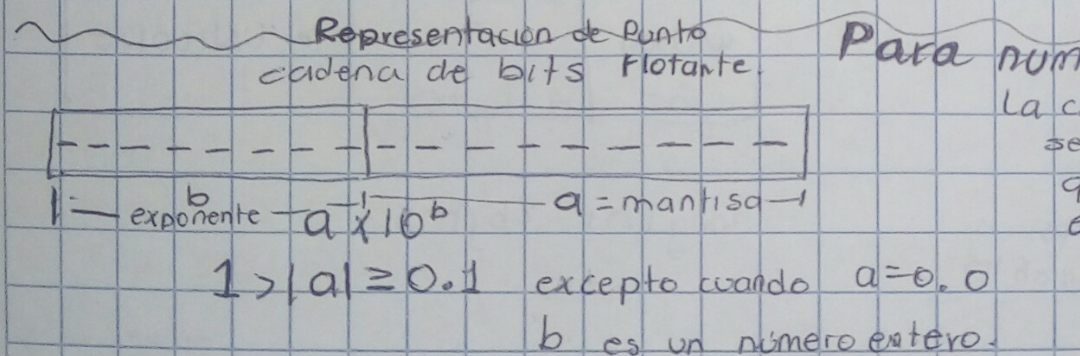
\includegraphics[scale=.16]{cadena-de-bits}
\centering
\caption{Cadena de bits.}
\end{figure}

\begin{center}
$a \times 10^b$\\
$0.1 \leq |a| < 1$\\
exceptuando cuando: $a=0.0b$ \\ 
\bigskip
\begin{tabular}{| c | c |}
\hline
Tipo de datos & Espacio de almacenamiento\\
\hline 
float& 4 bytes\\
double & 8 bytes\\
long double & 16 bytes\\
\hline
\end{tabular}
\end{center}

\section{Tipos de error}

\subsection{Error de corte}
Depende de la m\'aquina, es un error num\'erico,. P\'erdida de cifras significativas cuando sumamos o restamos cantidades con diferente orden de magnitud.\\
%poner ejemplo%

Epsil\'on de la m\'aquina (EPS): Es el n\'umero m\'as pequeño tal que $(1+EPS)\textgreater1$ para la m\'aquina que realiza la suma.
El siguiente c\'odigo permite conocer el epsil\'on de tu computadora.
\medskip
\begin{verbatim}
double EPS=1.0;
int k=0;
while((EPS+1.0)>1.0){
      EPS/=2.0;
      K++
      }
EPS*=2.0;
K--;
printf("Epsilon de la maquina = %f", EPS);
printf("\n Equivalente a 2^ %d", k);
\end{verbatim}

\subsection{Error de redondeo} 
P\'erdida de cifras decimales a medida que se aumenta el exponente.

%----Ilustración de recta-----%
\begin{figure}[h]
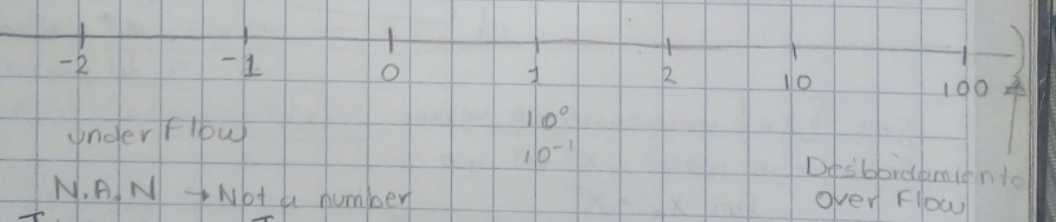
\includegraphics[scale=.16]{recta-error-redondeo}
\centering
\caption{Recta que ejemplifica el error de redondeo.}
\end{figure}

\subsection{Error de truncamiento}
Son aquellos que resultan al usar una aproximaci\'on en lugar de un procedimiento matem\'atico exacto.\\
Ejemplo:\\
Teorema de Taylor: Si $f(x)$ es una funci\'on suave en un intervalo abierto $(a,b)$ que contiene a $c$, para un n\'umero $c+h$ contenido en $(a,b)$ \\
$f(c+h)=f(c)+f'(c)h+f''(c)\frac{h^2}{2!}+f'''(c)\frac{h^3}{3!}+...+f^n(c)\frac{h^n}{n!}$ \\
El hecho de perder cifras debido a limitar el resultado a ciertas decimales es a lo que llamamos error de truncamiento.\\

\subsection{Complejidad algor\'itmica y costo computacional}
%---Diagramas---%

\begin{center}
\textbf{Tiempo de tendencia a funciones}\\
\begin{tabular}{| c | c |}
\hline
$\log(n)$ & \\
$n$ & Tiempos lineales \\ 
$n\log(n)$ & \\
\hline
$n^2$ & \\
$n^3$ & Tiempos polin\'omicos \\ 
$n^4$ & \\
\hline
$2^n$ & NP-Duro \\
$n!$ & NP-Cmpleto\\
\hline
\end{tabular}
\end{center}
%-Ilustracion de grafica log-%
\begin{figure}[h]
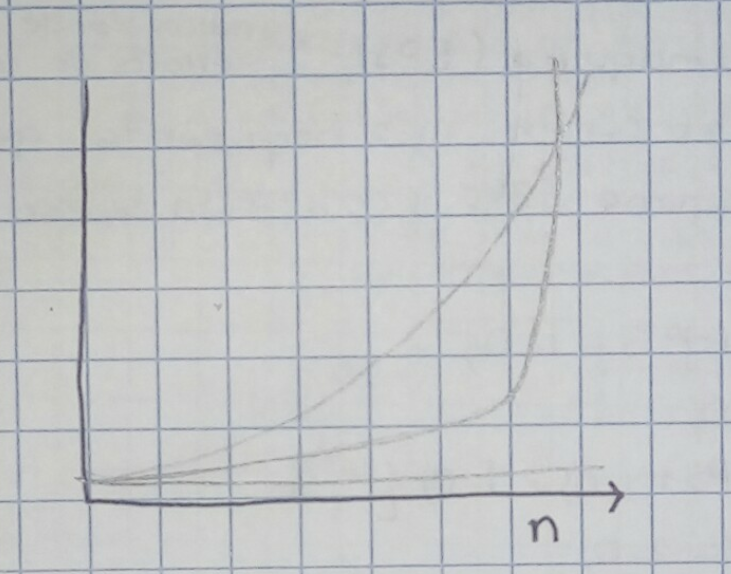
\includegraphics[scale=.16]{grafica-log}
\centering
\caption{Gr\'afica que estaba junto a lo de "Tiempo de tendencia de funciones".}
\end{figure}

\subsection{Convergencia} 
Un ciclo de c\'alculo se traduce a una iteraci\'on. \\

%--Ilustración de iteración--%
\begin{figure}[h]
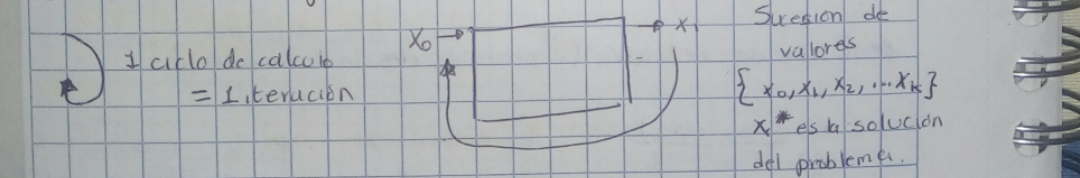
\includegraphics[scale=.16]{iteracion}
\centering
\caption{Iteraci\'on.}
\end{figure}

Sea $x_k$ una sucesi\'on de valores. Si existe un n\'umero $x^*$ tal que $$\lim\limits_{k\to\infty}x_k=x^*$$ \\
La sucesi\'on converge a $x^*$, si eso no ocurre, entonces la sucesi\'on diverge.\\
\\
\textbf{Velocidad de convergencia}\\ 
%--Ilustración de iteración--%
\begin{figure}[h]
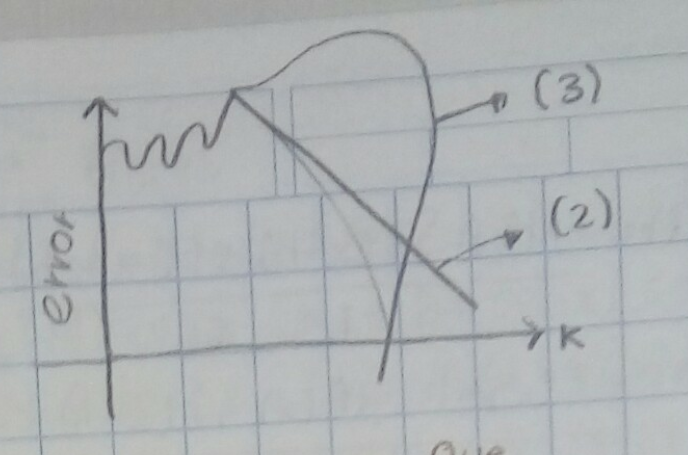
\includegraphics[scale=.16]{grafica-junto-vel-conv}
\centering
\caption{No estoy muy segura de la raz\'on de ser de la gr\'afica, pero estaba a un lado.}
\end{figure}

${x_k}$ converge a $x^*$ \\
\begin{enumerate}
\item Si existe un $k\geq 1$ a partir del cual se observa que $|x_{k+1}-x^*|\leq C|x_k-x^*|$ donde $C$ es constante entre $(0,1)$ se tiene velocidad de convergencia lineal.
\item Igual que el anterior pero $|x_{k+1}-x^*|\leq c_k|x_k-x^*|$ con $c_k\exists(0,1)$ y $C_k\to0$ cuando $k\to\infty$, se tiene  velocidad de convergencia lineal.
\item A partir de la iteraci\'on $k$ se observa que $|x_{k+1}-x^*|\leq C{|x_k-x^*|}^P$ donde $C$y $P$ son constantes $C\in(0,1)$ y $P\geq2$, se tiene convergencia de orden $P$.
\end{enumerate}

